\documentclass{tufte-handout}
\usepackage[utf8]{inputenc}
\usepackage[T1]{fontenc}
\usepackage[ngerman]{babel}
\usepackage{graphicx}

\usepackage{courier}
\usepackage{listings}
\lstset{
	language=python,
	basicstyle=\small\ttfamily,
	showstringspaces=false,
	numbers=left,
	frame=tb,
	literate={ä}{{\"a}}1 {Ä}{{\"A}}1 {á}{{\'a}}1 
		{é}{{\'e}}1 
		{ö}{{\"o}}1 {Ö}{{\"O}}1
		{ü}{{\"u}}1 {Ü}{{\"U}}1 
		{ß}{{\ss}}1
	}

%\setcounter{secnumdepth}{0}

\title{guizero}
\date{}
\author{Marco Bakera (bakera@tbs1.de)}

\begin{document}

\maketitle

guizero\footnote{https://lawsie.github.io/guizero} ermöglicht die einfache
Gestaltung von graphischen Benutzeroberflächen.
Es kann mit pip installiert werden.
\begin{marginfigure}
 Windows: pip install guizero\\ \noindent
 Linux/Mac: pip3 install guizero
\end{marginfigure}
  
Auf der Webseite wird eine alternative Möglichkeit der Installation
vorgestellt, die mit einem Download auskommt.
 
 
Die folgende Beispielanwendungen zeigen verschiedene GUI-Elemente in Aktion.
Der Quelltext muss ausgeführt werden, um das Fenster zu sehen. 
 
Zunächst ein leeres Fenster ohne Inhalt.

\begin{marginfigure}[3cm]
	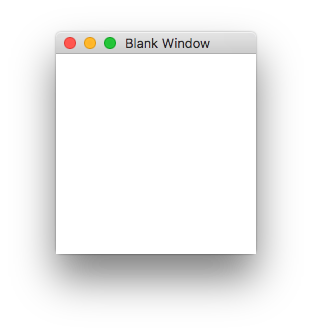
\includegraphics[width=\textwidth]{../blank_window}
\end{marginfigure}

\begin{figure}
\begin{lstlisting}
import guizero

class BlankWindow:
    def __init__(self, title="Blank Window"):
        self.root = guizero.App(title=title)

    def run(self):
        self.root.display()

w = BlankWindow()
w.run()
\end{lstlisting}
\end{figure} 

Nun ein Fenster mit einem Button. Die Methode \lstinline|click| wird bei einem
Klick auf den Button ausgeführt.

\begin{marginfigure}[3cm]
	\begin{center}
	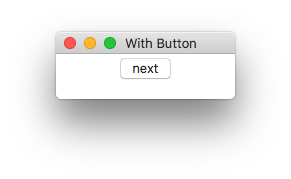
\includegraphics[width=\textwidth]{../with_button.png}
	\end{center}
	
	Ausgabe:
	\texttt{\\
Button clicked!\\ 
Button clicked!
}

	
\end{marginfigure}

\begin{figure}
	\begin{lstlisting}
class WindowWithButton(BlankWindow):
    def __init__(self):
        super().__init__("With Button")
        # add button, invoking method 'click' when clicked.
        btn = guizero.PushButton(self.root, text="next", 
                                 command=self.click)

    def click(self):
        print("Button clicked!")


w = WindowWithButton()
w.run()   	\end{lstlisting}
\end{figure} 

\clearpage

Zwei Buttons können in einem
Grid-Layout\footnote{https://lawsie.github.io/guizero/layout/} angeordnet
werden.

\begin{marginfigure}
	\begin{center}
		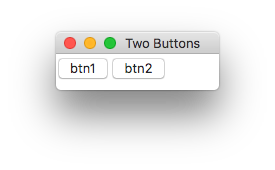
\includegraphics[width=\textwidth]{../with_2_buttons.png}
	\end{center}	
\end{marginfigure}

\begin{figure}
\begin{lstlisting}
class WindowWithTwoButtons:
    def __init__(self):
        self.root = guizero.App(title='Two Buttons', 
                                layout='grid')
        btn1 = guizero.PushButton(self.root, text="btn1",
                                  grid=[0,0])
        btn2 = guizero.PushButton(self.root, text="btn2",
                                  grid=[1,0])
    def run(self):
        self.root.display()

w = WindowWithTwoButtons()
w.run()

\end{lstlisting}
\end{figure} 

Die Klasse \lstinline|Picture| kann genutzt werden, um Bilder
anzuzeigen.\footnote{
	https://lawsie.github.io/guizero/images/} Hierfür wird ein
Bild mit einem Ball verwendet.

\begin{marginfigure}
	\begin{center}
		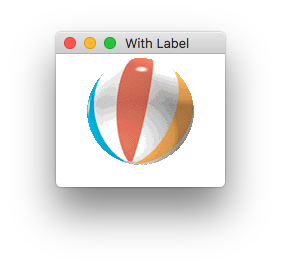
\includegraphics[width=\textwidth]{../with_label.png}
	\end{center}	
\end{marginfigure}

\begin{figure}
	\begin{lstlisting}
class WindowWithLabel(BlankWindow):
    def __init__(self):
        super().__init__("With Label")
        # add image in a Picture-Object
        self.bild = guizero.Picture(self.root,
                                    image="ball.gif")

w = WindowWithLabel()
w.run()
	
	\end{lstlisting}
\end{figure} 

\clearpage
Nun ein komplexeres Beispiel mit einem Menü, Button und Label.


\begin{marginfigure}[3cm]
	\begin{center}
		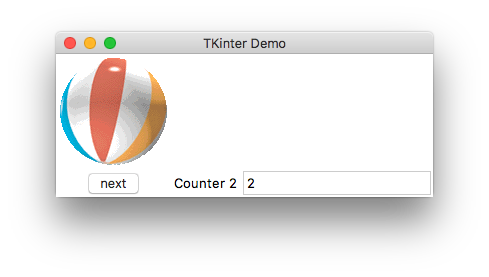
\includegraphics[width=1.2\textwidth]{../complex_demo.png}
	\end{center}	
\end{marginfigure}

\begin{figure}
	\begin{lstlisting}
class GUI:
    def __init__(self):
        self.counter = 0

        root = guizero.App(title='TKinter Demo', layout='grid')

        guizero.MenuBar(root,
                        toplevel=['Tools'],
                        options=[
                           [ ['Next', self.click] ]
                       ])
        # add image
        bild = guizero.Picture(root, image="ball.gif",
                               grid=[0,0])

        # add button, invoking method 'click' when clicked.
        btn = guizero.PushButton(root, text="next", 
                                 command=self.click,
                                 grid=[0,1])

        # add label with counter value
        self.lbl = guizero.Text(root, 
                                text="Label für Counter",
                                grid=[1,1])

        # add entry field
        self.ent = guizero.TextBox(root, grid=[2,1])

        # entering main event loop
        root.display()

    def click(self):
        # update label and counter
        self.lbl.value = "Counter %s" % self.counter
        self.counter += 1


GUI()	
\end{lstlisting}
\end{figure} 
 
\end{document}

